\cleartooddpage[\thispagestyle{empty}]
\renewcommand{\thefootnote}{\fnsymbol{footnote}}
\newcommand{\thetamc}{\theta_{\textrm{MC}}}
\newcommand{\mlratio}{$\left [ \frac{M_\odot}{L_\odot} \right ]$}
\chapter{The Dark Matter Paradigm}\label{ch_dm}

Dark matter makes up 26.5\% of the universe's energy and 81.5\% of its mass~\cite{planck2015}.
It has had a {\color{red}significant impact (which impact?? -maria)} on the development of the universe, shaping its present day distribution.
This chapter discusses the astrophysical evidence for the existence of dark matter, an outline of the current cosmological paradigm of $\Lambda$CDM and the Standard Model, as well as arguments for why dark matter may be in the form of a new, unknown particle.

%From: https://arxiv.org/abs/1502.01589 , Table 3, column [4] :
%  omega_b h^2 = 0.02225
%  omega_c h^2 = 0.1198
%  H_0         = 67.27 km / s / Mpc
%  h           = H_0 / ( 100 km / s / Mpc ) = 0.6727
%thus:
%  omega_b = 0.02225 / h^2 = 0.0491 =  4.9% of universe's energy is in baryonic matter
%  omega_c = 0.1198  / h^2 = 0.2647 = 26.5% of universe's energy is in dark matter
%  ( 26.5 - 4.9 ) / 26.5 = 81.5% of universe's mass is stored in dark matter

\section{Astrophysical Evidence for Dark Matter}
  
The current effects attributed to dark matter can be grouped into four different length scales.
On the smallest length scales, groups of several thousand stars can be seen revolving around their center of mass.
By measuring the doppler-shift of their spectral lines, they are observed to be moving at wider distribution of speeds than one would expect from the existing visible amount of matter.
At larger scales the optical light from galaxies, as well as hydrogen lines, can be used to measure the amount of mass and its rotational velocity around the center of galaxies.
At even larger scales, galaxy velocities can be measured and compared, X-ray telescopes can monitor the amount of hot gas, and mass-heavy areas of space will gravitationally lens background galaxies.
At the largest scale, the measurement of oscillations in the cosmic microwave background can be used to determine the amount of dark and baryonic matter.
These effects can all be generalized to observations of gravity pulling on electromagnetic emitters, gravity bending background light, and the universe's total energy budget.

Throughout this chapter, astrophysical objects are measured in units of the Sun's mass $M_\odot$, and the Sun's luminosity $L_\odot$.
For these conversions, nominal values are $M_\odot =$ \SI{1.9885e30}{kg} and $L_\odot =$ \SI{3.828e26}{W}, though different authors may use slightly different values depending on the year of publication~\cite{iau_solarconstants}.
The amount of dark matter in an object is then expressed in terms of the ratio $\frac{\textrm{M}_\odot}{\textrm{L}_\odot}$.
For example, a ratio of \SI{7}{\frac{M_\odot}{L_\odot}} indicates that for every \SI{1}{M_\odot} worth of mass producing light (at a rate similar to the Sun), theres another \SI{6}{M_\odot} of mass in a dark form.
  
\subsection{Scales of $10^{19}\:\text{m}$ : Dwarf Galaxies}\label{dm_dwarfscale}
% 10^19m comes from: 
% fornax dwarf spheroidal galaxy wiki page
%    17' x 12.6' in solid angle, call it 15'
%    140kpc away  
%    140kpc * Tan(15') = 0.6kpc = 1.8*10^19m ~ 10^19m
At scales of $\nicetilde 10^{19}$m, groups of thousands stars, called satellite galaxies or dwarf galaxies, lie at the edge of full size galaxies like our own.
These dwarf galaxies are strong evidence for dark matter because their luminous matter is not enough to gravitationally bind them.
An example of two dwarf galaxies are shown in Figures~\ref{fig:sculptor} and \ref{fig:fornax}.
Figure~\ref{fig:sculptor} is the Sculptor dwarf galaxy, imaged in the optical frequencies by the MPG/ESO Telescope, while Figure~\ref{fig:fornax} is the Fornax dwarf galaxy, from the ESO Digitized Sky Survey II~\cite{fornax_image}.

\begin{figure}[!ht]
  \centering
  \includegraphics[width=0.8\textwidth]{images/sculptor/sculptor.eps}
  \caption[Sculptor Dwarf Galaxy]{
    The Sculptor dwarf galaxy~\cite{sculptor_image}, with a $\frac{M_\odot}{L_\odot}$ ratio of $15.3\pm6.9$~\cite{sculptor_ml}, imaged by the MPG/ESO telescope~\cite{sculptor_paper}.
  }
  \label{fig:sculptor}
\end{figure}

\begin{figure}[!ht]
  \centering
  \includegraphics[width=0.8\textwidth]{images/fornax/fornax.pdf}
  \caption[Fornax Dwarf Galaxy]{
    The Fornax dwarf galaxy, with a $\frac{M_\odot}{L_\odot}$ ratio of $8.8\pm3.8$~\cite{sculptor_ml}, from the ESO Digitized Sky Survey II~\cite{fornax_image}.
  }
  \label{fig:fornax}
\end{figure}

Measuring the mass of these dwarf galaxies is done in two ways.
In the first, telescopes observed the individual spectra of these stars, allowing for their line-of-sight velocity to be calculated~\cite{dwarf_gal_red_giant}.
The width of the distribution of the velocities is called the velocity dispersion.
By looking at this velocity dispersion, the total mass of the dwarf galaxy can be inferred~\cite{dwarf_gal_vel_dispersion, dwarf_gal_vel_dispersion2}.
What makes this possible is that the velocity dispersion of a group of stars is proportional to the total mass of the gravitational well.

This is derived from the spherical Jean's equation, shown by Equation~\ref{eqn:jeans}~\cite{galactic_dynamics},

\begin{equation}\label{eqn:jeans}
  \frac{d}{dr} \left ( v \sigma_r^2\right) + \frac{2 \beta}{r}v \sigma_r^2 + v \frac{d \Phi}{dr}=0 \;\; ,
\end{equation}

where $r$ is the distance from the center of mass, $v(r)$ is a 3D distribution of stars, $\Phi(r)$ is a gravitational potential, $\sigma_r(r)$ is the distribution of radial velocities, and $\sigma_\theta(r)$ is the distribution of velocities orthogonal to the $r$ direction.
The parameter $\beta = 1 - \frac{\sigma_{\theta}^2}{\sigma_r^2}$ characterizes how different the two velocity distributions ($\sigma_r(r)$ and $\sigma_{\theta}(r)$) are.
A solution to this equation can be used to calculate the measurable line-of-sight velocity distribution $\sigma_{\mathrm{los}}$ as a function of the projected angle from the center-of-mass of the dwarf $R$, shown in Equation~\ref{eqn:los_velocity_dist},

\begin{equation}\label{eqn:los_velocity_dist}
  \sigma_{\mathrm{los}}^2 \left ( R \right ) = \frac{2}{I(R)} \int_R^{\infty} \left ( 1 - \beta(r) \frac{R^2}{r^2}) \right ) \frac{r}{\sqrt{r^2-R^2}} \frac{1}{f(r)} \int_r^\infty f(s) \frac{v(s)GM(s)}{s^2} \; ds\; dr \;\; ,
\end{equation}

with

\begin{equation}\label{eqn:los_velocity_dist2}
  f(r) = f_{r'} \exp \left [ \int_{r'}^r \frac{2 \beta(t) }{t} \; dt \right ] \;\; .
\end{equation}

In Equations~\ref{eqn:los_velocity_dist} and \ref{eqn:los_velocity_dist2}, $I(R)$ is the surface brightness of the dwarf galaxy, $v(s)$ is the density profile of its luminous component, $M(s)=4\pi \int_0^s \rho_{\textrm{DM}}(r) r^2 \; dr$ the enclosed dark matter mass, and $\beta(r)$ velocity anisotropy profile.
The calculated $\sigma_{\mathrm{los}}(r)$ velocity distribution in Equation~\ref{eqn:los_velocity_dist} can then be compared to the radial velocity measurements of stars within dwarf galaxies to estimate the total mass (dark + baryonic)~\cite{dwarf_gal_vel_dispersion,dwarf_gal_vel_dispersion_a,dwarf_jfactors_no_priors}.
As stellar velocity measurements rely on doppler-shifted spectral lines, and not the star's absolute brightness, any derived mass estimates are fairly robust with respect to changes in observed brightness.
These changes in brightness can be from atmospheric variations during telescope observations or changes in the amount of light-absorbing dust in the line-of-sight.

The second way to measure galaxy masses is by measuring the total brightness of a galaxy, and divide by the luminosity of the Sun $L_\odot$.
This then indicates the number of solar masses $M_\odot$ contained in the galaxy, a measure of its baryonic (i.e. 'bright', not dark) mass.
% from https://arxiv.org/pdf/1510.07674.pdf
% L_\odot from page 3, table "SOLAR CONVERSION CONSTANTS" 
% M_\odot :
%   G*M_\odot = 1.3271244e20 m^3 s^-2 (from table "SOLAR CONVERSION CONSTANTS")
%   G = 6.67408e-11 m^3 kg^-1 s^-2
%   thus 
%   M_\odot = 1.3271244e20 m^3 s^-2 / 6.67408e-11 m^3 kg^-1 s^2
%           = 1.98847e30 kg
    
The first way measures the `total' mass from the rotational profile, while the second only measures the mass of its 'luminous' parts.
The ratio of the 'total' mass divided by the 'luminous' mass is called the mass-to-light ratio, which indicates the amount of dark matter present in the galaxy~\cite{faber_ml}.
Dwarf galaxies have mass-to-light ratios of around 5-100 $\frac{M_\odot}{L_\odot}$, but can reach up to \nicetilde \SI{1000}{\frac{M_\odot}{L_\odot}}~\cite{Simon2007_dwarfgalaxykeck}.
These high values are considered strong evidence in favor of dark matter.
A random assortment of Local Group dwarf galaxies and their $\frac{M_\odot}{L_\odot}$ is shown in Table~\ref{tab:mlratios:dwarfgals}.
    
\begin{table}[h]
  \centering
  \caption[Ratios of $\frac{M_\odot}{L_\odot}$ for Various Dwarf Galaxy Objects]{
    Ratios of $\frac{M_\odot}{L_\odot}$ for various dwarf galaxy objects~\cite{localdwarfs}.
  }
  \label{tab:mlratios:dwarfgals}
  \begin{tabular}{l r | l r | l r | l r}
    Object      &  \mlratio{} & Object & \mlratio{} & Object & \mlratio{} & Object & \mlratio{} \\
    \hline
    IC 10       &  0.1 & NGC 147    &  7.1 & Sagittarius & 22 & Leo I    &  3.1 \\
    NGC 185     &  2.5 & NGC 205    & 12   & Ursa Minor  & 60 & Fornax   &  4.8 \\
    LGS 3       & 21   & IC 1613    &  1.4 & Draco       & 58 & Sculptor & 11   \\
    Carina      & 30   & Antlia     &  7.4 & Sextans     & 34 & GR 8     &  8.3 \\
  \end{tabular}
\end{table}
% from reference \cite{localdwarfs}, table 4, (M/L)_{0,V}^i column
    
As an additional piece of evidence for dark matter, dwarf galaxies near the Perseus cluster were studied.
From the gravitational potential of their baryonic mass alone, these dwarf galaxies should be ripped apart by the tidal disruption of the Perseus cluster.
Instead, observations of these dwarf galaxies indicate they remain intact, leading to the conclusion that the presence of dark matter is providing extra gravitational force~\cite{Penny2009}.

\FloatBarrier

\subsection{Scales of $10^{20}\:\text{m}$ : Galaxies}\label{dm_gal}
%
% galaxy rotation curve wiki page, M33 has curve measurements out to 50,000ly
%   50,000ly = 4.7*10^20m ~ 10^20m
At scales of $\nicetilde 10^{20}$m, some effects of dark matter on galaxies are also observable.
Within galaxies, the amount of light observed in a sector predicts a lower amount of mass, while observing the line-of-sight velocity predicts a higher amount of mass.

In the first prediction technique, the total amount of light produced by a quadrant of a galaxy is measured with optical telescopes.
Then, as in Section~\ref{dm_dwarfscale}, the amount of light produced can be compared with the Sun as a standard mass-to-light ratio, allowing for a prediction of the amount of mass contained in that sector.
Known mass-to-light ratios can then be used to calculate the total amount of mass within that quadrant.
For example, in a survey of 25 galaxies in Ref. \cite{galaxy_mass_light_ratio}, most possesed a mass-to-light ratio of 1 to 10.

In the second prediction technique, a galaxy's emission spectrum is observed at many positions around its disk (center, outer edges, etc).
By comparing the orientation of the disk with the doppler-shifted position of well-known spectral lines, one can calculate the average velocity that each section is traveling at around the center of its galaxy, forming a rotation curve~\cite{rotation_curve_review, spiral_galaxy_rot_curve, milkyway_dm_evidence}.
Newton's law of gravity can then be used to calculate the mass contained within a sphere of that same radius.
This calculation results in a larger amount of mass than the one found simply from the total amount of light observed.

In Figure~\ref{fig:m33rotcurve}, a rotation curve from M33 observations is shown.
The observed velocity curve (the datapoints) continues to increase at larger radii.
If the galaxy was only made of stars, then the rotation curve would follow the short dashed line.
If the galaxy was only made of gas, then the rotation curve would instead follow the long dashed line.
As these two major components do not combine to form the observed rotation curve, the presence of dark matter can account for the difference, shown as the dashed-dotted line~\cite{m33rotcurve}.
    
\begin{figure}[!t]
  \centering
  \includegraphics[width=0.8\textwidth]{images/m33rotcurve/m33rotcurve.eps}
  \caption[M33 Rotation Curve]{
    The rotation curve from M33~\cite{m33rotcurve}.
    The solid line is the best fitting model to the observed velocity measurments.
    The short dashed line is the stellar disk contribution, the gas contribution is the long dashed line, and the dashed-dotted line is the dark matter contribution.
  }
  \label{fig:m33rotcurve}
\end{figure}

\begin{table}[h]
  \centering
  \caption[Ratios of \mlratio{} for Various Galactic-scale Objects]{Ratios of $\frac{M_\odot}{L_\odot}$ for various galactic-scale objects~\cite{faber_ml}.}
  \label{tab:mlratios}
  \begin{tabular}{l r | l r}
    Object      &  \mlratio{} & Object & \mlratio{} \\
    \hline
    M31 (Andromeda) &  7.6  & NGC 801  &  2.4  \\
    M33             &  4.5  & NGC 2403 &  5.5  \\
    M51             &  3.3  & NGC 2841 & 10.6  \\
    M81             &  8.5  & NGC 4324 &  5.5  \\
    M83             &  2.3  & NGC 6822 &  0.58 \\
  \end{tabular}
\end{table}
% values from Ref. \cite{faber_ml}, Table 1, M/L_B column
      
A random sample of galaxies from Ref. \cite{faber_ml} are shown alongside their mass-to-light ratios in Table \ref{tab:mlratios}.
Our own Milky Way galaxy is measured to have a mass to light ratio of \SIrange{1.2}{1.5}{\frac{M_\odot}{L_\odot}}~\cite{milkyway_ml_ratio} {\color{red}(orel would remove this whole sentence??)}.

Further evidence of dark matter can be deduced through additional weak gravitational lensing~\cite{weak_lensing_2001}.
Lensing elliptical galaxies can constrain mass profiles, as the amount of lensing indicates the total amount of mass, which in turn limits the amount of dark matter present at different radii~\cite{weak_lensing_ellipse}.

\begin{figure}[!b]
  \centering
  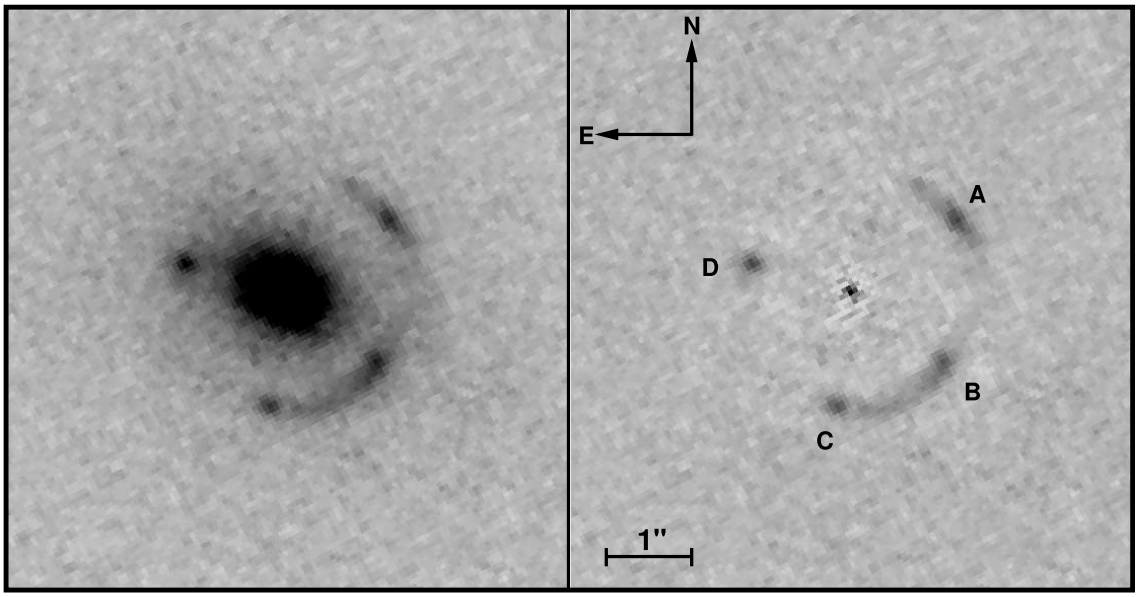
\includegraphics[width=0.8\textwidth]{images/weak_lensing_ellipse/weak_lensing.pdf}
  \caption[Weak Lensing with an Ellipse Galaxy]{
    Galaxy 0047-281 imaged by the Hubble Space Telescope, from Ref. \cite{weak_lensing_ellipse}.
    Left: Original image.
    Right: Same as Left but with the central foreground galaxy subtracted, leaving behind 4 lensed images A, B, C, and D of a background galaxy.
  }
  \label{fig:ellipse}
\end{figure}
    
Galaxy lensing can be used to estimate the size of the substructure of a lensing galaxy.
In the case of Galaxy 0047-281 in Figure~\ref{fig:ellipse}, the galaxy's mass bends light from a background quasar.
This creates 4 images of the background quasar~\cite{weak_lensing_quasar}.
The spectra of the four lensed images vary in brightness and distortion.
These variations can be seen by looking at the ratio of the widths of different spectral lines.
These ratios of different lensed images indicate that there exists variations in the mass density in the lensing galaxy.
%These variations are best fit by randomly distributing spheres of lensing mass throughout the lensing galaxy, each having a mass of \SI{10^6}{\Msol}.
These variations are best fit by randomly distributing spheres of lensing mass throughout the lensing galaxy, each having a mass of \SI{e6}{\Msol}.
Spheres of this mass are consistant with the scale of dark matter substructure predicted by CDM.

\subsection{Scales of $10^{23}\:\text{m}$ : Galaxy Clusters}\label{dm_galclusters}
%
% galaxy cluster wiki page
% 2-10 Mpc, call it 6Mpc = 1.85*10^23m ~ 10^23m
At scales of $\nicetilde 10^{23}$m, dark matter's effects on galactic clusters become observable with several techniques.
In one technique, the mass-to-light ratio can be measured for galaxy clusters.
This is done the same as with dwarf galaxies; luminous mass is derived from the brightness of the cluster, while total mass is measured from the velocity dispersion of individual galaxies within the cluster.
From measurements of several hundred galaxy clusters, it was found that galaxy clusters have mass-to-light ratios of \SIrange{10}{1000}{\frac{M_\odot}{L_\odot}}~\cite{cluster_ml_ratios}, indicating a very high amount of dark matter is present in these objects.
Several galaxy clusters and their $\frac{M_\odot}{L_\odot}$ ratios are shown in Table~\ref{tab:cluster_ml_ratios}.

\begin{table}[h]
  \centering
  \caption[Ratios of \MLsol for Various Galaxy Clusters]{
    Ratios of \MLsol for various galaxy clusters~\cite{cluster_ml_ratios}.
    }
  \label{tab:cluster_ml_ratios}
  \begin{tabular}{l r | l r | l r}
    Object & \mlratio{} & Object & \mlratio{} & Object & \mlratio{} \\
    \hline
    Abell   85 & 445 & Abell 2426 &  80 & Abell 3695 & 180 \\
    Abell  458 & 401 & Abell 3122 & 960 & Abell 3921 & 175 \\
    Abell  999 & 100 & Abell 3126 & 491 & Abell 4008 & 227 \\
    Abell 1228 &  37 & Abell 3354 &  94 & Abell 4053 & 421 \\
  \end{tabular}
\end{table}
    
Another technique for measuring the total mass is by examining the amount of gravitational lensing caused by a cluster.
When a massive galaxy cluster has a galaxy directly behind it, the image of the background galaxy gets distorted.
The shape of the distorted image can then be used to infer the amount of total mass in the galaxy cluster.
Then comparing this total mass to the luminous mass provides an estimate for the amount of dark matter contained in the galaxy cluster.
This was used with galaxy clusters Abell 370 and CL 2244-02 to estimate the amount of dark matter in each~\cite{cluster_lensing}.
Lensing cluster Abell 370 and several distorted background galaxies are shown in Figure~\ref{fig:abell370}.
This technique found that for both Abell 370 and CL 2244-02, a large amount of dark matter is required to fit the observed arcs, within the range of 200-1000 \MLsol.
    
\begin{figure}[!ht]
  \centering
  \includegraphics[width=0.8\textwidth]{images/abell370/abell370_cropped.pdf}
  \caption[Gravitational Lensing in Abell 370]{
    Galaxy cluster Abell 370 is shown here, along with many gravitationally lensed background galaxies.
    The large arc marked by the green lines is the distorted background galaxy image used to calculate the cluster's total mass~\cite{cluster_lensing}.
    Credit: NASA, ESA/Hubble, HST Frontier Fields~\cite{abell370_hubble}.
  }
  \label{fig:abell370}
\end{figure}
    
Another example of using gravitational lensing to measure dark matter mass is with cluster Cl0024+1654.
This galaxy cluster creates several lensed images of the same background galaxy, which are used to measure the total mass.
The lensing is shown in Figure~\ref{fig:stronglens}, where the blue arcs are the distorted background galaxy images.
From all of these lensed images, the best fit amount of dark matter indicates this cluster has a mass-to-light ratio of \SI{161}{}\MLsol{}\footnote[3]{This measurement scales with the hubble constant, which here is assumed to be \SI{70}{km/s/Mpc}}~\cite{cluster_strong_lensing_1996, cluster_strong_lensing_1998, cluster_strong_lensing_2010}.
%assumes a hubble constant of 70\SI{230}$\,h_{70}\,$\MLsol, where $h_{70}$ is set to $0.70$
    
\begin{figure}[!ht]
  \centering
  \includegraphics[width=0.8\textwidth]{images/cluster_strong_lensing_8/stronglensing2.pdf}
  \caption[Gravitational Lensing in Cl0024+1654]{
    Strong lensing of a blue background galaxy by galaxy cluster Cl0024+1654 into multiple blue distorted images~\cite{cluster_strong_lensing_1996}.
  }
  \label{fig:stronglens}
\end{figure}
    
Yet another way of measuring the total mass of a cluster is by examining X-ray measurements.
In galaxy clusters, the majority of the luminous mass is stored in warm ($kT\simeq\,$\SI{5}{keV}) gas, rather than stars.
This warm gas emits X-rays, which can be detected by satellites like Chandra~\cite{chandra}.
By measuring the X-ray flux at the center of the galaxy cluster Abell 2029, the total mass of the cluster can be estimated.
This is done by assuming the warm gas is in hydrostatic equilibrium, where the force of gravity towards the cluster center is equally balanced by the pressure of the warm gas.
This implies that when moving outwards from the cluster center, the density and temperature of the gas is predictable.
From this, the mass-to-light ratio can be inferred at several different radii from the cluster center.
Within \SI{28.5}{kpc}\footnote[2]{This scales inversely with the hubble constant, assumed here to be \SI{70}{km/s/Mpc}} of the center, the ratio is 12 \MLsol, while beyond a radius of \SI{286}{kpc}\footnotemark[2] the ratio rises above 100 \MLsol{}, indicating a high amount of dark matter is present~\cite{cluster_chandra}.

These previously mentioned techniques have been combined into an analysis of galaxy cluster {\color{red}1E 0657-558 (maria highlited this??)} to provide a cardinal piece of evidence in favor of particle dark matter.
This cluster consists of two subgroups of galaxies, a larger 'target' cluster, and a smaller Bullet cluster.
Each cluster's mass is contained in two clouds; gas and stars that form the baryonic cloud, and the much more massive dark matter cloud.
The baryonic cloud is visible through Chandra X-ray observations, which is able to image the warm ($kT\simeq\,$\SI{10}{keV}) gas and infer its density.
The dark matter cloud is inferred through weak lensing observations, where the mass of the cluster distorts the images of background galaxies.
In this pair of clusters, the Bullet cluster has fallen through the target cluster.
However, the two clouds of the Bullet cluster dragged on the clouds of the target cluster, and dragged at different rates.
This difference in drag over time resulted in a separation between the Bullet cluster's baryonic and dark matter clouds, visible in Figure~\ref{fig:bullet}.

\begin{figure}[!ht]
  \centering
  \includegraphics[width=0.95\textwidth]{images/bulletcluster/bulletcluster_cropped.pdf}
  \caption[The Bullet Cluster]{
    The Bullet Cluster~\cite{bullet_cluster_combined_image}.
    The blue clouds indicate the graviational lensing mass~\cite{bullet_cluster}, the pink represents clouds of warm gas emitting X-rays~\cite{bullet_cluster_chandramap}.
    The red triangle indicates the bullet cluster's warm gas center-of-mass, and the blue oval marks the approximate center of the weak lensing (dark) mass.
    The remaining stars and galaxies are imaged in the optical spectrum~\cite{bullet_cluster_composite}.}
  \label{fig:bullet}
\end{figure}
    
The pink clouds are X-ray observations of the cluster's warm gas, while the blue clouds are the weak lensing mass.
The red triangle and blue oval show the approximate centers of mass of the bullet cluster's two clouds.
The difference in position between the two centers of mass allows for constraints to be put on the dark matter particle's mass and cross section.
This contraint is shown in Equation~\ref{eqn:bullet}, where $\sigma_{\chi}$ is the dark matter particle cross section, and $m_{\chi}$ is the dark matter particle mass~\cite{bullet_cluster,bullet_cluster2},

\begin{equation}\label{eqn:bullet}
  \frac{\sigma_{\chi}}{m_{\chi}} < 1 \, \textrm{cm}^2 \, \textrm{g}^{-1} \;\; .
\end{equation}

%This result was improved by combining 72 galaxy cluster collisions, improving the limit in Equation~\ref{eqn:bullet} to \SI{0.47}{cm^{2} g^{-1}}~\cite{cluster_72}.
Further work on this combined 72 galaxy cluster collisions, improving the limit in Equation~\ref{eqn:bullet} to \SI{0.47}{cm^2 g^{-1}}~\cite{cluster_72}.


\subsection{Scales of $10^{26}\:\text{m}$ : The Observable Universe and $\Lambda$CDM Cosmology}\label{dm_universe}
%\subsection{Inter-Cluster Scale}
% age of universe (13.82*10^9 years * speed of light) = 1.307*10^26m
At the universe's largest scale, $\nicetilde 10^{26}$m, the Cosmic Microwave Background (CMB) has been used to measure the total amount of dark matter in the universe.
By looking at the structure of the CMB, the structure of the universe and its particle populations can be studied, including how they developed and changed from the Big Bang to the present day.
In order to understand dark matter's place in the evolution of the universe, several important moments must be discussed.

The first moment of the universe was Inflation, where a singularity with a temperature of $kT=10^{17}\:\textrm{GeV}$ quickly expanded as a quark-gluon plasma and cooled~\cite{inflation0,inflation1,inflation2,inflation3}.
Once the average temperature had reduced enough, quarks could bind together to form baryons, in a stage known as Baryogenesis.
The time/temperature that Baryogenesis occurred at has not been determined.
However, there are several competing theories that may explain how an unequal ratio of baryons to antibaryons were created~\cite{baryogenesis1,baryogenesis2}.

Later on when the universe is around \nicetilde380,000 years old and has expanded enough to cool to \nicetilde\SI{3000}{K}, another phase change can occur.
Here, the universe is a sea of photons ($\gamma$), electrons, and protons.
With all the free electrons and protons around, the mean free path of the photon is small, so they are in thermal equilibrium with the electrons and protons.
Once the universe expands further, enough to cool below the electron-proton binding energy, electrons start being captured by protons in great numbers.
Since electrons and protons have formed electrically neutral hydrogen atoms (an event called recombination), the universe becomes transparent to these photons, which are then free to travel the universe~\cite{planck2015,theEarlyUniverse,CMBFundamentals,CMBFlat}.
The spectrum of these photons follows a blackbody spectrum, shown in Figure~\ref{fig:cmb_black}, and is called the cosmic microwave background.

\begin{figure}[ht]
  \centering
  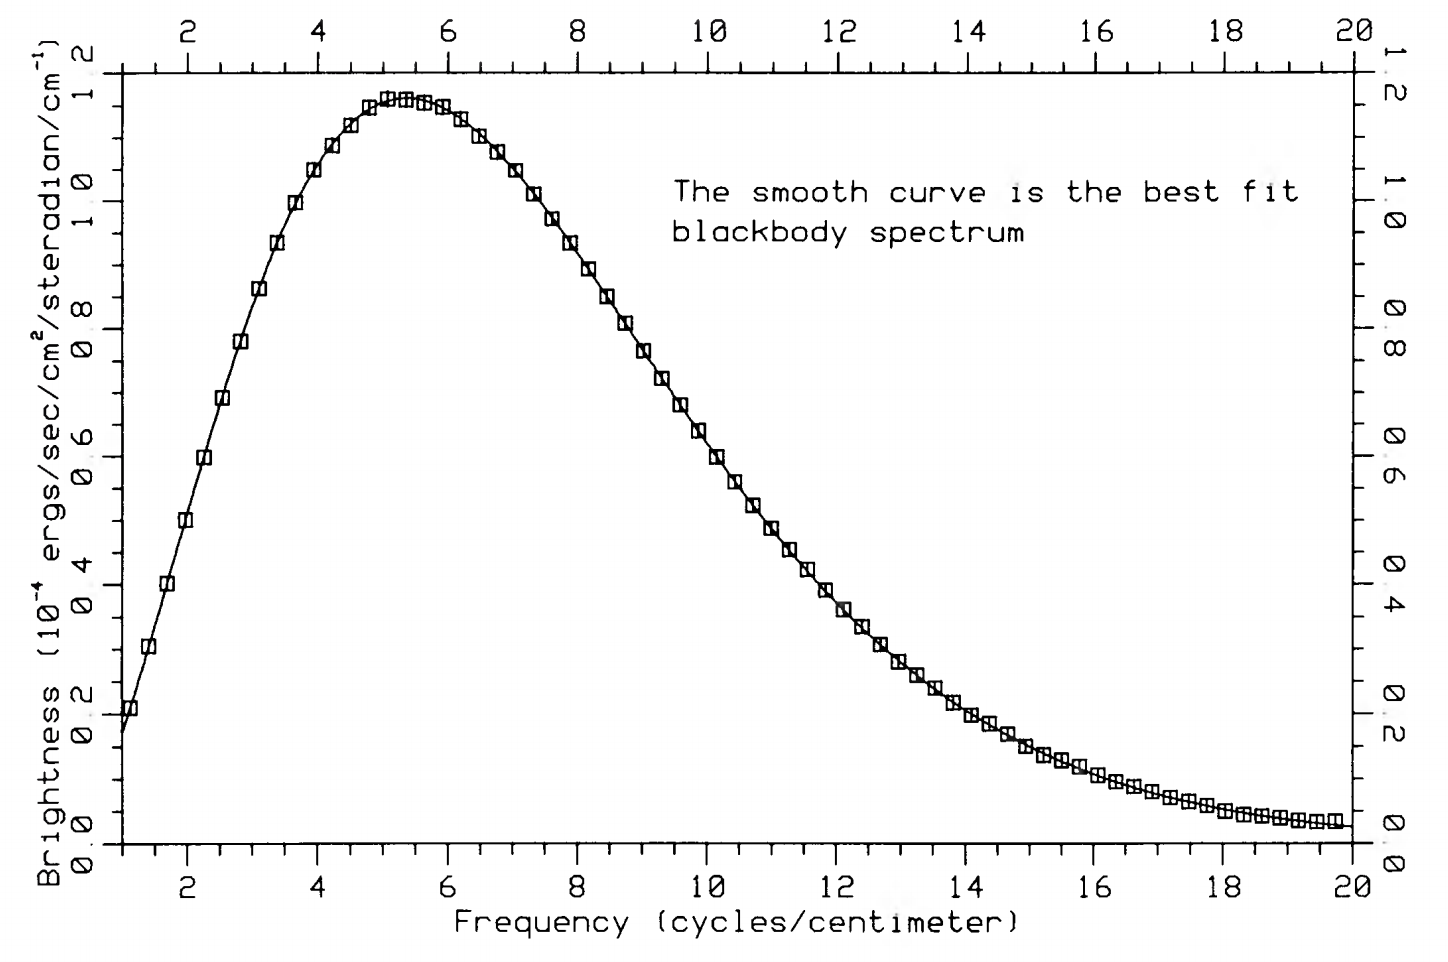
\includegraphics[width=0.85\textwidth]{images/cmb_blackbody/cmb.pdf}
  \caption[Cosmic Microwave Background Blackbody]{
    The blackbody spectrum of the cosmic microwave background measured by the FIRAS instrument on the COBE satellite~\cite{mather1990}.
    Errorbars shown are from an assumed 1\% error.
  }
  \label{fig:cmb_black}
\end{figure}

\begin{figure}[ht]
  \centering
  \includegraphics[width=0.95\textwidth]{images/cmb_skymap/cmb_skymap.eps}
  \caption[Cosmic Microwave Background Skymap]{
    The cosmic microwave background temperature map of the universe \cite{wmap_skymap}, from 9 years of WMAP observations~\cite{wmap9year}.
    The colors span a temperature range of \SI{\pm200}{\mu{}Kelvin}.
  }
  \label{fig:cmb}
\end{figure}

However, the CMB spectrum varies a small amount from a pure blackbody spectrum, roughly 1 part in 1000, in different parts of the sky.
% cmb temp varies 2.7260 +- 0.0013
% Fixsen, D. J. (2009). "The Temperature of the Cosmic Microwave Background", arxiv 0911.1955
% 2.7260/0.0013 = ~2000 ~=  1 in 1000
These variations are shown in Figure~\ref{fig:cmb}, and are due to Baryon Acoustic Oscillations (BAOs), which were imprinted when the electrons and protons recombined.
This recombination was not an instantaneous event however, and instead happened over time.
During this gradual recombination, some baryons were gravitationally pulled into areas of higher mass densities.
These high-density areas were formed in earlier times of the universe, and were spread out evenly.
The baryons would fall into these gravitational wells, until they became warmer, whereupon the baryons emit more photons, which increases the photon pressure and drives the baryons out of the wells.
Eventually after leaving the wells, the photon pressure decreases and the gravitiational force takes over, drawing the matter back towards the gravitational wells again.
After happening repeatedly, this created ripples of density waves (acoustic oscillations), which spread outwards, interferring with one another.
These density waves, which had dense high-temperature areas, and sparse low-temperature areas, then emitted blackbody photons at higher and lower temperatures, respectively.
These higher and lower temperatures account for the spectrum of variations in the CMB's temperature in different parts of the sky.

As the CMB is emitted by scattering off the baryons, the CMB spectrum only depends on the baryon temperature.
However, since the baryons were pulled into the high density areas by gravity, the presence of dark matter increases the wavelength of these density ripples.
This is similar to a simple spring pendulum, where adding an extra (dark) mass to an existing (baryonic) mass will decrease the oscillation frequency ($\omega = \sqrt{\frac{k}{m}}$), resulting in BAOs with longer wavelengths.
Thus, by measuring the wavelength of the BAOs with the CMB correlations, the amount of dark matter in the universe can be estimated.
The CMB correlation spectrum, measured by Planck, is shown in Figure~\ref{fig:cmb_correlation_spectra}.

\begin{figure}[t]
  \centering
  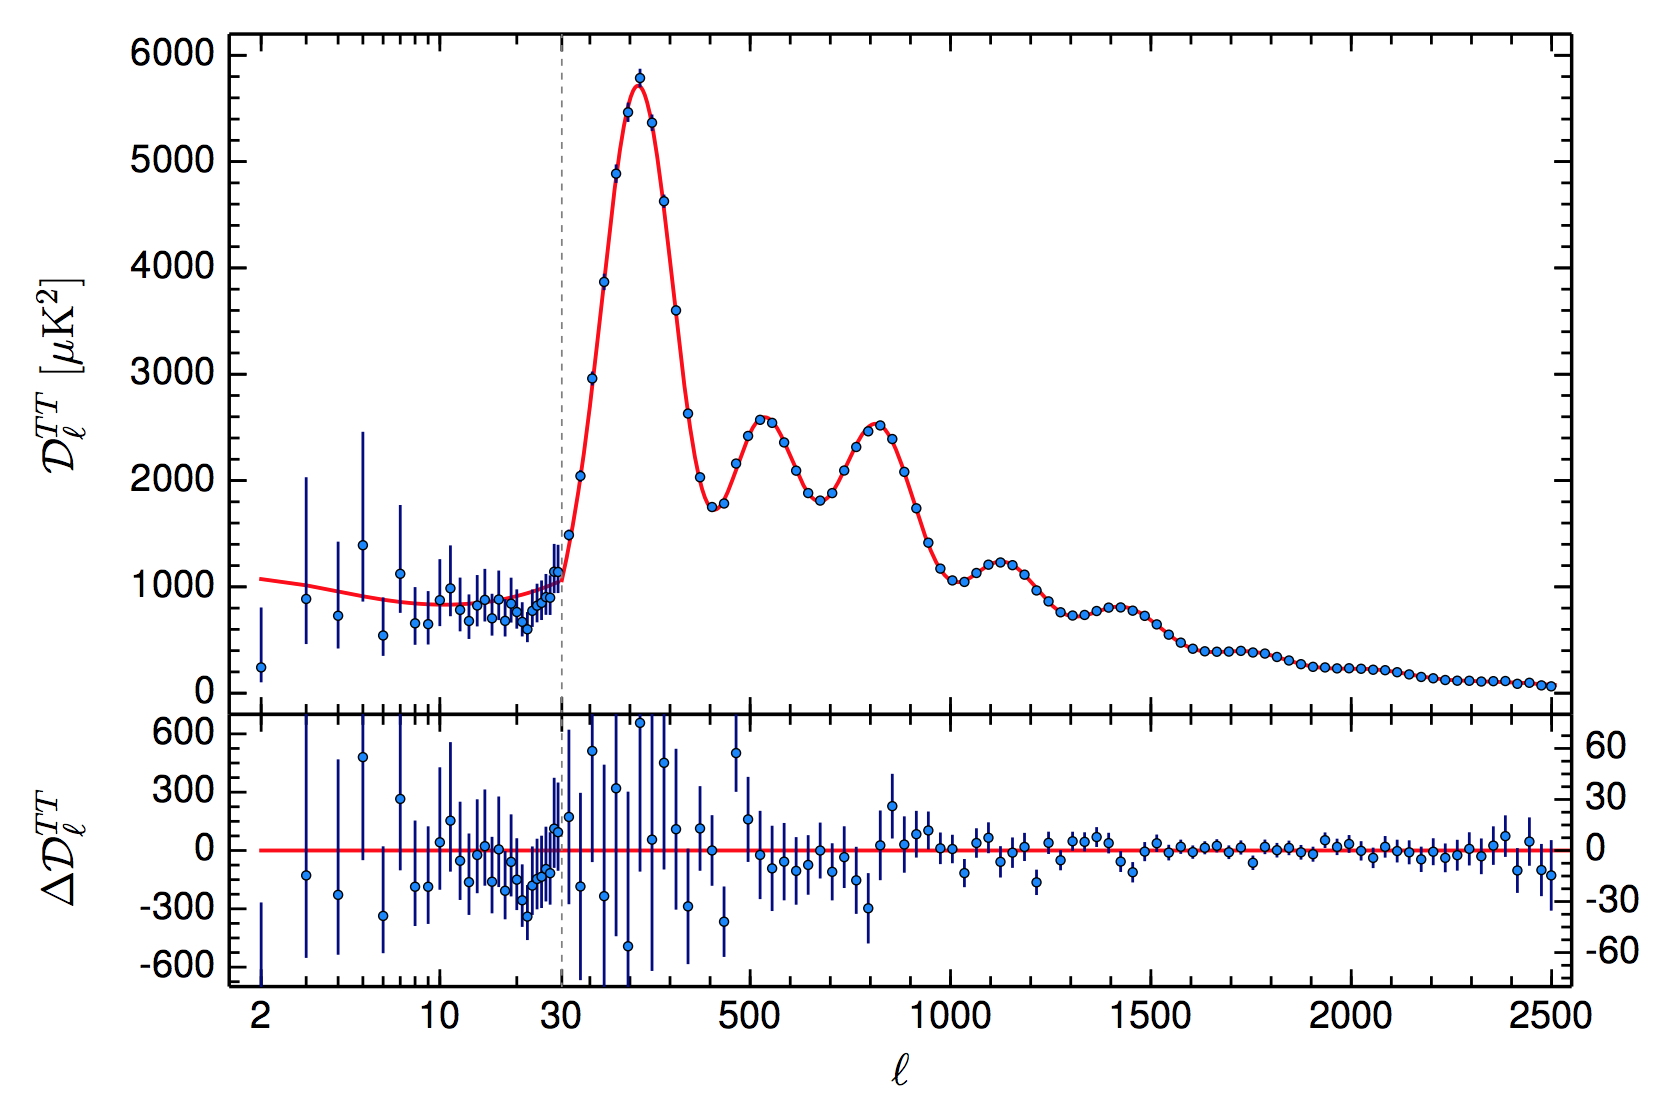
\includegraphics[width=0.85\textwidth]{images/cmb_spectra_planck_2018/cmb_spectra.pdf}
  \caption[Cosmic Micrwave Background Correlation Spectrum]{
    Correlation spectra from CMB temperature measurements with the Planck satellite~\cite{planck_dm_limit}.
    The upper plot shows the spectra, the lower panel shows the residuals.
  }
  \label{fig:cmb_correlation_spectra}
\end{figure}

From the BAOs in Figure~\ref{fig:cmb_correlation_spectra}, it has been found that 68.6\% of the universe is stored in Dark Energy, a repulsive force which causes almost all visible galaxies to accelerate away from each other.
% 100% - ( 26.5% + 4.9 ) = 73.5% (from beginning of chapter)
Another 4.9\% of the universe's energy is stored in baryonic matter, like protons and neutrons.
The remaining 26.5\% of the universe's energy is contained in dark matter~\cite{planck2015}.

The polarization of CMB photons also incorporates information about dark matter and its properties.
The CMB photons come from ambient photons that Thompson-scattered off electrons right before recombination.
Because of this Thompson scattering, the CMB photons inherit both temperature and polarization information.
Dark matter annihilations during recombination may produce standard model particles, which act as an injection of ionization energy, extending the duration of recombination.
A longer recombination acts to decrease any CMB temperature fluctuations while increasing CMB polarization fluctuations~\cite{cmb_polarization1,cmb_polarization2}.
{\color{red}(this paragraph is missing the result from CMB polarization studies, no?? -orel)}
% first polarization discovery: 
%   Detection of polarization in the cosmic microwave background using DASI
%   http://adsabs.harvard.edu/abs/2002Natur.420..772K

The measurements of the CMB contribute to the existing theory of how the universe developed after the Big Bang, called $\Lambda$CDM.
The $\Lambda$ refers to the density of dark energy, while CDM refers to Cold Dark Matter.
This theory predicts the different times particles froze out of the universe, and their resulting distributions.

% from planc 2018 results cosmological constants, table 1
% hubble constant :
%   H_0 = (67.4+-0.5) km/s/Mpc
%   h = H_0 / 100 km/s/Mpc = 0.674
% \Omega_b h^2 = 0.02233 +- 0.00015
%   \Omega_b = 0.02233 / h^2 = 0.02233 / 0.674^2 = 0.04915 -> 4.915 +- 0.033 %
% \Omega_c h^2 = 0.1198 +- 0.0012
%   \Omega_c = 0.1198  / h^2 = 0.1198  / 0.674^2 = 0.2637  -> 26.37 +- 0.264 %
% ln( A_s * 10^10 ) = 3.043 +- 0.014
%   A_s = e^(3.043+-0.014) * 10^-10 = (2.097+-0.029)*10^-9
%   

\begin{table}[t]
  \centering
  \begin{tabular}{llcl}
               & \textbf{Value}                 & \textbf{Unit} & \textbf{Description} \\
    \hline 
    $\Omega_b$ & $ 4.915  \pm0.033                 $ & \%       & Universe's energy in Baryons \\
    $\Omega_c$ & $ 26.37  \pm0.264                 $ & \%       & Universe's energy in Dark Matter \\
    $\thetamc$ & $(1.04089\pm0.00031)\times 10^{-2}$ & Radians  & Angular size of the sound horizon \\
    % from https://github.com/cmbant/CosmoMC/blob/master/paramnames/params_CMB.paramnames :
    %   "the ratio of the angular diameter distance to the LSS sound horizon"
    $\tau$     & $(5.40   \pm0.74   )\times 10^{-2}$ & unitless & Thompson scattering optical depth (opacity)\\
    % arxiv: 0205436 , section II, 3rd paragraph
    $A_s$      & $(2.097  \pm0.029  )\times 10^{-9}$ & unitless & Seed density spectrum amplitude \\
    $n_s$      & $ 0.9652 \pm0.0042                $ & unitless & Seed density spectrum spectral index \\
    \hline 
  \end{tabular}
  \caption[6 Cosmological Parameters]{
    The best fit values for the six cosmological parameters using CMB measurements, from Ref.~\cite{planck_dm_limit}}
  \label{tab:six_params}
\end{table}

From the CMB correlation spectrum in Figure~\ref{fig:cmb_correlation_spectra}, six parameters that describe the universe can be modelled~\cite{planck_dm_limit,planck_2013_parameters}.
These are shown in Table~\ref{tab:six_params}.
The parameters $\Omega_b$ and $\Omega_c$ are the fraction of the universe's energy stored in baryons and cold dark matter, respectively.
The parameter $\thetamc$ is the angular range that could be influenced during the BAOs produced after recombination.
This is the comoving distance a sound wave could have traveled between the beginning of the universe and recombination.
The parameter $\tau$ describes how opaque the universe became to photons during reionization, where the first stars started to reheat atoms and free electrons.
The parameters $A_s$ and $n_s$ govern the amplitude and the spectral index of the initial seed perturbations in the early universe.
These universe-scale parameters determine how the universe evolved over time.

The observed quantities of deuterium in the early universe also hint at dark matter's properties.
During Big Bang Nucleosynthesis when the universe was only a few seconds old, protons and neutrons were starting to combine into various isotopes, one of which is deuterium.
However, like baryons, the amount of deuterium produced in the early universe is heavily dependent on the initial baryon number density.
So, any constraint on the deuterium fraction is also a constraint on the baryon fraction of the universe~\cite{deuterium1,deuterium2}.
From the spectrum of deuterium and hydrogen lines from the quasar QSO Q0913+072, the baryon fraction was measured to be $\Omega_{b}h^2 = 0.0224 \pm 0.0005$~\cite{deuterium3}, indicating only 4.93\% of the universe's energy is stored in baryons.
% h = 0.674 (see below)
% 0.0224 / h^2 = 0.0224 / 0.674^2 = 0.0493 -> 4.93% of universe's energy
This suggests that only a small amount of matter in the universe can be made of baryons, and the rest must instead reside in some non-baryonic form.
{\color{red}(not sure I understood where dark matter comes into play here.  Is it the density I marked?? Can this be clarified without adding too much? -orel)}

Another measurement that depends heavily on the presence of dark matter is the rate at which galaxies cluster together.
In the Sloan Digital Sky Survey (SDSS), the positions of 1.6 million galaxies, quasars, and stars are mapped~\cite{sdss_release}.
By simulating the distribution of similar objects as the universe ages, the rate that galaxies cluster together can be measured, which depends on the total mass of all objects in the field of view.
Only with extra mass from dark matter does the universe form clumps that match SDSS observations.

Because dark matter is likely a new, undiscovered particle, a discussion of particle physics and the Standard Model is necessary to understand what properties a new dark particle may possess.

\section{The Standard Model}

The current paradigm of particle physics is called the Standard Model~\cite{standardmodel}.
It consists of groups of particles called quarks and leptons, as well as the bosons that mediate interactions between these particles.
Quarks combine to form hadrons, like protons and neutrons, and mesons, while leptons consist of electrons, muons, tauons, and their neutrino companions.

At the forefront of dark matter search candidates are particles predicted by Supersymmetry~\cite{Jungman:1995df}, (specifically Minimal Supersymmetric Standard Model, or MSSM~\cite{MSSM,supersym1}), an extension to the Standard model.
Much like how most particles have an anti-particle, in supersymmetry, each Standard Model quark, lepton, and boson has a supersymmetric partner particle.
Quarks and leptons have squarks and sleptons as their supersymmetric partners, while bosons have partners like gluinos, and charginos.
While no evidence of supersymmetry has been discovered to date, it is still preferred due to its ability to predict physics across a large range energy scales, the holy grail of any Grand Unified Theory.


\subsection{Particle Dark Matter}\label{sec_particledm}

Early in the search for a candidate dark matter particle, Standard Model (SM) particles were first considered.
One dark matter candidate was the neutrino, due to how many there are in the universe and their lack of interaction with the strong and electromagnetic forces.
This was generally referred to as Hot Dark Matter, as neutrinos travel at relativistic speeds.
However, it was eventually demonstrated that because of these relativistic speeds, neutrinos would diffuse out of their initial overdensities.
This would result in large super-cluster-scale gravitational wells forming first, then cluster-scale wells, then galaxy-scale wells, called top-down structure formation.
When observations are made of earlier times, the opposite is found: galaxy-scale gravitational wells form first, then cluster-scale wells, then super-cluster-scale wells in present times, called bottom-up formation.
As this is the opposite of what is expected for relativistic dark matter, neutrinos were ruled out as a dark matter candidate~\cite{neutrinoHeirarchical}.
% from this discussion: https://physics.stackexchange.com/questions/158319/why-are-neutrinos-ruled-out-as-a-major-or-even-sole-component-of-dark-matter

In addition, limits on the mass of the neutrino ($\sum{}m_{\nu} = 0.194 \; \textrm{eV}, \; 95\% \; \textrm{C.L.}$) also rule it out since they are not numerous enough~\cite{planck2015}.
% see table 5, sum m_nu [eV] row, TT, TE, EE+lensing+ext column
All other Standard Model particles have also been ruled out, usually for reasons of charge, mass, number density, or cross section.
Since none of the Standard Model particles meet the conditions to be a dark matter candidate, theoretically predicted particles are now the focus of most searches.

One of the major expansions to the Standard Model that may contain a dark matter candidate is Supersymmetry, or SUSY.
There are several SUSY extensions, but the main one discussed here is the Minimal Supersymmetric Standard Model (MSSM)~\cite{MSSM,supersym1,schelke_thesis}.
The basic idea of SUSY is that, just as majorana fermions have a particle-antiparticle reflection, SUSY adds another reflection called R-parity for all particles. 
This R-parity is defined as

\begin{equation}
  R = (-1)^{3B+L+2S}
\end{equation}

where $B$ is the baryon number, $L$ is the lepton number, and $S$ is the particle spin.
This creates supersymmetric partner particles (superpartners) for each Standard Model particle, usually denoted by an 's-' prefix or an '-ino' suffix added to a particle name, and \nicetilde{} added atop the particle symbol ($e \rightarrow \tilde{e}$).
Quarks become squarks, leptons become sleptons, and gluons become gluinos, etc.
Standard model particles and fields have an R-parity of +1, while superpartners have an R-parity of -1.

When this SUSY reflection is performed, the superpartners develop some interesting properties.
The superpartners all have their spin reduced by $\frac{1}{2}$, so the fermionic electron with spin $\frac{1}{2}$ becomes a bosonic selectron with spin $0$, and the bosonic gluon with spin 1 becomes the fermionic gluino with spin $\frac{1}{2}$.
When the $W^{\pm}$  and weak hypercharge are reflected, they form the Bino and the Wino, respectively.
When the Higgs field is reflected, two Higgsino fields result.
The Bino, Wino, and two Higgsino fields then mix together to form 4 new particles called neutralinos.
The lightest of these neutralinos has some properties that make it an excellent dark matter candidate, and is the WIMP candidate ($\chi$) searched for in this thesis.
Specifically, as it is the lightest neutralino, other neutralinos will decay into it.
If R-parity is conserved, then this neutralino will also be stable, and not decay into anything else~\cite{neutralino1,neutralino2,neutralino3}.
These two features would give the neutralino the stability to exist until the present day, and the numbers needed to match predictions from dark matter observations.

\subsection{Relic Freezeout and WIMP Miracle}

%This means it would be able to exist since the freezeout without significant losses to its population
The relic freezeout refers to how dark matter may have behaved in the past.
A population of dark matter particles existed during the early universe (a relic particle), and that at a later time the universe expanded enough that their numbers stopped changing (the freezeout).

This freezeout is relevant because it hints at the self-interacting cross section of the WIMP.
Early on when the universe was still expanding, its been theorized that WIMPs were annihilating into SM particles, and SM particles were interacting and producing WIMPs.
The number density and cross section of these two particle populations were such that that the number of WIMPs and SM particles remained constant; the two particle populations were in thermal equilibrium.

As the universe expanded, both particle groups ran into each other less and less.
This meant that fewer particles were converted to the opposite population, meaning temperature changes in one population took longer and longer to propagate to the other population.
Eventually the two populations became independent, sometimes called thermal decoupling.
After this decoupling, WIMPs continued to annihilate occasionally, further reducing their numbers, until there were so few left that they stopped encountering each other.
As the population of WIMPs likely did not change much after that time, it is called a freezeout.

The Boltzman equation describing how the number of WIMPs evolves through this freezeout is,

% some of this derivation is from https://ned.ipac.caltech.edu/level5/March10/Garrett/Garrett7.html
%   for example, this is equation 20:
\begin{equation}\label{eqn:boltzmann_relic}
  \frac{dn}{dt} = - 3 H n \: - \left \langle \sigma_{A} v \right \rangle \left ( n^2 - n_{eq}^2 \right ) \;\;,
\end{equation}

where $n$ is the comoving WIMP number density, $H$ is the hubble expansion rate ($\frac{\dot{a}}{a}$), $\left \langle \sigma_{A} v \right \rangle$ is the effective velocity-averaged cross section for $\chi\chi$ annihilating into standard model particles~\cite{wells_relic}.
The parameter $n_{eq}$ is the equilibrium WIMP comoving number density.

\begin{figure}[!ht]
  \centering
  \includegraphics[width=0.75\textwidth]{images/relic_abundance_plot/updated.pdf}
  \caption[Relic Abundance vs Time]{
    The relic abundance of WIMPs as a function of temperature, from Ref.~\cite{updatedWIMPRelicCrossSection}, where $m$ is the WIMP mass.
    The universe's temperature is $T$, which decreases as the universe expands.
    Therefore $x$ is a proxy for time, increasing as one moves to the right along the x-axis.
    The number of WIMPs in a comoving volume is $n(x)$, $n_{\textrm{eq}}(x)$ is the number of WIMPs at equilibrium, and the y values are scaled by $n_{\textrm{eq}}(x=1)$.
    The weak, electromagnetic (em), and strong cross sections are shown for a \SI{100}{\GeV{}} WIMP, with additional lines for the weak cross section at \SI{1}{\GeV{}} and \SI{e3}{\GeV{}}.
    The cross sections shown are:
    \begin{tabular}{ll}
    $\left \langle \sigma v \right \rangle_{\textrm{weak}}  $  & $= 2 \times 10^{-26} \; \textrm{cm}^3 \textrm{s}^{-1}$ \\
    $\left \langle \sigma v \right \rangle_{\textrm{em}}    $  & $= 2 \times 10^{-21} \; \textrm{cm}^3 \textrm{s}^{-1}$ \\
    $\left \langle \sigma v \right \rangle_{\textrm{strong}}$  & $= 2 \times 10^{-15} \; \textrm{cm}^3 \textrm{s}^{-1}$ \\
    \end{tabular} .
  }
  \label{fig:abundance}
\end{figure}

Equation~\ref{eqn:boltzmann_relic} is numerically solved and shown in Figure~\ref{fig:abundance}.
It shows how the number of WIMPs evolve as the universe ages, and its temperature decreases.
The black equilibrium line indicates the number of WIMPs that would be left if they had a large ($\left \langle \sigma v \right \rangle >> 2 \times 10^{-15} \textrm{cm}^3 \textrm{s}^-1$) cross section.
This black line shows how the populations of SM particles annihilating into WIMPs and visa versa balance and replenish each other, forming an equilibrium number density.
As the cross section decreases, fewer and fewer particles are annihilated, and more of the initial WIMP population survives to freeze out.
This freezeout can be thought of as the universe expanding faster than the particles can annihilate.

The cross section of WIMPs can then be estimated from Equation~\ref{eqn:boltzmann_relic}.
If the total amount of dark matter is known, and its mass estimated, this indicates the number density of WIMP particles present in the universe.
This number density combined with Equation~\ref{eqn:boltzmann_relic} then indicates the cross section of a \SI{100}{\GeV{}} WIMP to be around $\left \langle \sigma_{\chi} v \right \rangle \approx 3 \times 10^{-27} \textrm{cm}^{3}\textrm{s}^{-1}$

An interesting coincidence is that the weak cross section of a \SI{100}{\GeV{}} particle is approximately \SI{e-25}{cm^3s^{-1}}, only two orders of magnitude away from the cross section found from the relic abundance~\cite{Jungman:1995df}.
{\color{red}(As far as I remember, and a quick Wikipedia search confirms (not the best source, I know), the cross-section for both WIMP and weak interaction 100 GeV particle is ~$10^{-26}$. So they are much closer than the two orders of magnitude you discuss here. Am I remembering it wrong?? -orel)}
This is quite surprising, as the cosmology of the relic abundance and the weak cross section come from very different physics.
While this is not conclusive proof of the WIMP's existence, this \textit{WIMP Miracle} is intruiging physics to search for.

As the motivation for dark matter searches is now understood, a search can be prepared.
The next question is ``How does one look for dark matter?''.
If one has access to a gamma-ray observatory, it turns out dark matter annihilations may produce observable gamma rays.
So, the next chapter discusses how a cloud of dark matter around the Galactic Center might create an observable spectrum of gamma rays, and how those gamma rays can be detected at Earth.

